% id: 0520
% book: 쎈 중3-2 수학 · 05 원주각의 활용
% section: 유형 02 원에 내접하는 사각형의 성질 (1)
% figure: tikz:fig-0520
% answer: ④
% answer_source: 답지
% variant_level: 0 (원본 전사)
% 이 파일은 build.mjs 가 items.json 에서 만든다. 고칠 때는 items.json 을 고친다.
\smash{\raisebox{1.5mm}{\dmkichul{쎈 중3-2 수학 0520번 · 94쪽}}}
\noindent\begin{minipage}[t]{0.58\linewidth}\vspace{0pt}\raggedright 오른쪽 그림과 같이 $\square\pt{ABCD}$가 원~$\pt{O}$에 내접하고 $\angle\pt{ABO}=55^\circ$, $\angle\pt{ADO}=20^\circ$일 때, $\angle\pt{C}$의 크기는?\end{minipage}\hfill\begin{minipage}[t]{0.4\linewidth}\vspace{0pt}\centering \resizebox{\ifdim\width>\linewidth\linewidth\else\width\fi}{!}{% 0520(본책 94쪽) — 원 O 에 내접하는 □ABCD, OB·OD, ∠ABO=55°, ∠ADO=20°, ∠C(색칠). 다시 그림.
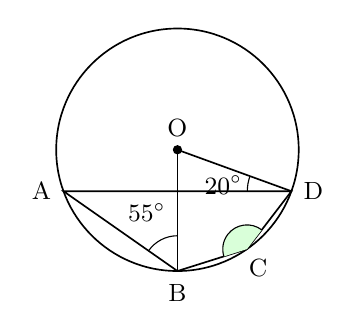
\begin{tikzpicture}[scale=1.40, line width=0.6pt]
  \draw (0.000,0.000) circle (1.100);
  \draw (-1.034,-0.376) -- (-0.000,-1.100) -- (0.631,-0.901) -- (1.034,-0.376) -- cycle;
  \draw (0.000,0.000) -- (-0.000,-1.100);
  \draw (0.000,0.000) -- (1.034,-0.376);
  \fill (0.000,0.000) circle (1.2pt);
  \draw[line width=0.4pt] (-0.000,-0.780) arc[start angle=90.000, end angle=145.000, radius=0.320];
  \node[font=\small, inner sep=0.5pt] at (-0.277,-0.568) {$55^\circ$};
  \draw[line width=0.4pt] (0.658,-0.239) arc[start angle=160.000, end angle=180.000, radius=0.400];
  \node[font=\small, inner sep=0.5pt] at (0.416,-0.322) {$20^\circ$};
  \fill[green!15] (0.631,-0.901) -- (0.765,-0.727) arc[start angle=52.500, end angle=197.500, radius=0.220] -- cycle;
  \draw[line width=0.4pt] (0.765,-0.727) arc[start angle=52.500, end angle=197.500, radius=0.220];
  \node[font=\small, inner sep=1.5pt] at (-1.234,-0.376) {A};
  \node[font=\small, inner sep=1.5pt] at (-0.000,-1.300) {B};
  \node[font=\small, inner sep=1.5pt] at (0.731,-1.074) {C};
  \node[font=\small, inner sep=1.5pt] at (1.234,-0.376) {D};
  \node[font=\small, inner sep=1.5pt] at (0.000,0.200) {O};
\end{tikzpicture}
}\end{minipage}\par
\begin{choicesii}{$136^\circ$}{$139^\circ$}{$142^\circ$}{$145^\circ$}{$148^\circ$}\end{choicesii}
